\documentclass[aps,reprint]{revtex4-1}
% Engine-specific settings
% Detect pdftex/xetex/luatex, and load appropriate font packages.
% This is inspired by the approach in the iftex package.
% pdftex:
\ifx\pdfmatch\undefined
\else
    \usepackage[T1]{fontenc}
    \usepackage[utf8]{inputenc}
\fi
% xetex:
\ifx\XeTeXinterchartoks\undefined
\else
    \usepackage{fontspec}
    \defaultfontfeatures{Ligatures=TeX}
\fi
% luatex:
\ifx\directlua\undefined
\else
    \usepackage{fontspec}
\fi
% End engine-specific settings
\usepackage[english]{babel}
\usepackage{csquotes}
% \usepackage[backend=bibtex, sortcites]{biblatex}
\usepackage{url}
\usepackage{textcomp}
\usepackage[usenames,dvipsnames,svgnames, table]{xcolor}
\usepackage[font={scriptsize}]{caption}
\usepackage{amsmath} \usepackage{amsthm} \usepackage{amsfonts}
\usepackage{amssymb}
\usepackage{enumerate}
\usepackage{tikz} \usepackage{float}
\usepackage[procnames]{listings}
\usepackage{pstool} \usepackage{pgfplots}
\usepackage{wrapfig} \usepackage{graphicx} \usepackage{epstopdf}
\usepackage{afterpage}
\usepackage{physics}
\usepackage{multirow}
\usepackage{gensymb}
\usepackage{algorithm}
\usepackage{microtype}
\usepackage[noend]{algpseudocode}
\usepackage{xcolor,colortbl}
\usepackage{microtype}
\usepackage{geometry}
\usepackage{hyperref}
\usepackage{graphicx}
\usepackage{caption}
\usepackage{subcaption}
\usepackage{lipsum}
% \usepackage{pythontex}
% \usepackage{authblk}
\usepackage{nth}
\usepackage{siunitx}
% \usepackage[toc,page]{appendix}
\floatstyle{plaintop}
\restylefloat{table}

% Custom commands
\newcommand{\unit}[1]{\:\mathrm{#1}}
\newcommand{\noref}[1]{\hyperref[#1]{\ref*{#1}}}
\newcommand{\nonref}[1]{\hyperref[]{\ref*{#1}}}
\newcommand\blankpage{%
  \null
  \thispagestyle{empty}%
  \addtocounter{page}{-1}%
  \newpage}

% Default fixed font does not support bold face
\DeclareFixedFont{\ttb}{T1}{txtt}{bx}{n}{7} % for bold
\DeclareFixedFont{\ttm}{T1}{txtt}{m}{n}{7}  % for normal

\newcommand\numberthis{\addtocounter{equation}{1}\tag{\theequation}}
\DeclareCaptionFont{white}{\color{white}}
\DeclareCaptionFormat{listing}{\colorbox{gray}{\parbox{\columnwidth}{#1#2#3}}}
\pgfplotsset{compat=1.14}


% Biber for references
\bibliographystyle{aipauth4-1}

\begin{document}
\sisetup{detect-all}
\title{Mimicking the flight of a Dipterocarpus fruit}
\author{Magnus Holm}
\author{Jonas G. S. Lunde}
\author{Frederik J. Mellbye}
\affiliation{University of Oslo, Oslo, Norway}
\date{\today}

\maketitle

\section{Introduction}
\label{sec:introduction}
See the lab instructions for a full introduction to this experiment. In the experiment
3D models of Dipterocarpaceae fruit were developed in FreeCAD, 3D-printed and
released in a water cylinder. The fruits are equipped with wings, which enables
seed dispersion over vast distances. The seed flight was then assessed with a
variety in important parameters such as fruit mass and wing curvature. Out of the
specific models that were investigated, ideal parameters for maximizing fruit
dispersion were determined.

\section{Theory}
\label{sec:theory}
\subsection{Non-dimensional quantities. Reynolds and Strouhal numbers.}
From the project description, there are nine physical variables which are based
on the dimensions $M$ (mass), $L$ (length) and $T$ (time). By Buckingham's
$\Pi$-theorem, there are
\begin{align*}
  p = n - k = 9 - 3 = 6
\end{align*}
dimensionless groups that can be constructed from the original variables.
Two of the possible $\Pi$-groups are the Reynolds and Strouhal numbers. Using
the nongeometrical parameters these can be written as
\begin{align}
  Re &= \frac{U_V L}{\nu}\\
  St &= \frac{fL}{U} = \frac{\omega L}{2\pi U}
\end{align}
\subsection{Expression for sinking velocity}
One might make the faulty assumption that only a reduced set of parameters influence the sinking velocity of an object in a fluid. Using, for instance, only the accelecation of gravity $g$, the surface area of the object $A$, the mass of the object $m$, and it's sinking velocity, one might construct the dimentionless group
\begin{align*}
    \Pi_1 = \frac{U_v^4}{g^2A}
\end{align*}
giving the proportionality
\begin{align*}
    U_v \sim g^{1/2}A^{1/4}
\end{align*}
This is obviously nonsense, and demonstrates the limitations of dimensional analysis when a reduced set of parameters are mistakenly used.

\subsection{Lift and drag forces on a wing element}
By the Kutta-Joukowski condition, for low angles of attack the lift is
proportional to (with inviscid theory)
\begin{align*}
    L \sim \rho U^2 L \sin{\alpha}
\end{align*}
This expression was found in Acheson, in the chapter on classical aerofoil theory.
In our case the velocity is given by $U = \omega R$, which yields a lift
\begin{align}
  L \sim \rho \omega^2 R^2 L
\end{align}
This formula might be inaccurate because in the experiment, viscous effects
created a trailing vortex. This is not accounted for by inviscid theory.

From dimensional analysis a possible configuration for the drag force is
\begin{align}
  D \sim \rho R^2 U_V \cos{\phi}
\end{align}
where we have taken the cosine of $\phi$ because if $\phi \rightarrow 0$ the
drag should increase and if $\phi \rightarrow \pi/2$ the drag should decrease.
This drag expression is both dimensionally and intuitively pleasing.
\subsection{Moment on the seed}
\label{subsec:moment}
When the moment is 0, there is no net torque on the seed. The pitch angle causes
fluid to be pushed to one side of the wing, which exerts a torque on the wings.
In turn, the higher rotational frequency increases lift and drag forces, as well
as viscous no-slip forces which counter the rotation and applies an opposite
torque. At some terminal velocity, the torques cancel out and the net moment is
0.

If the moment is 0 for a combination of vertical velocity $V_0$ and rotation
frequency $f_0$, the moment remains 0 if these quantities are multiplied with
some real constant $K$. This is because the Stouchal number remains constant,
so the rotation profile is the same (in a scaled sense).
\section{Experiment method}
The seeds were released in an approximately two meter tall glass cylinder filled
with water. This was repeaded twice for each combination of seed type and mass.
A raising mechanism was available to allow for easy recovery of the falling
seeds, except for a two mistakes in which the seeds were manually retreived with
a stick from the bottom of the tank. The seed trajectories were measured with
a web-camera for later analysis.

Several python scripts handed out were used to analyze the videos. Quantities
such as seed and wing positions (and hence rotation) over time were extracted
from the videos.
\label{sec:method}
\section{Results and discussion}
\label{sec:results}
See figures ~\ref{fig:oppg1} and ~\ref{fig:oppg2} for results from the
experiment.
\begin{figure}
  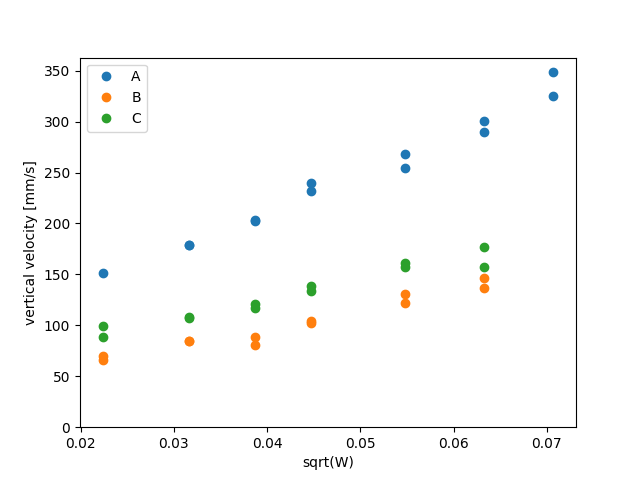
\includegraphics[width=0.8\linewidth]{oppg1.png}
  \caption{
    \label{fig:oppg1}
    Vertical velocity of the differents seeds at different masses
  }
\end{figure}
\begin{figure}
  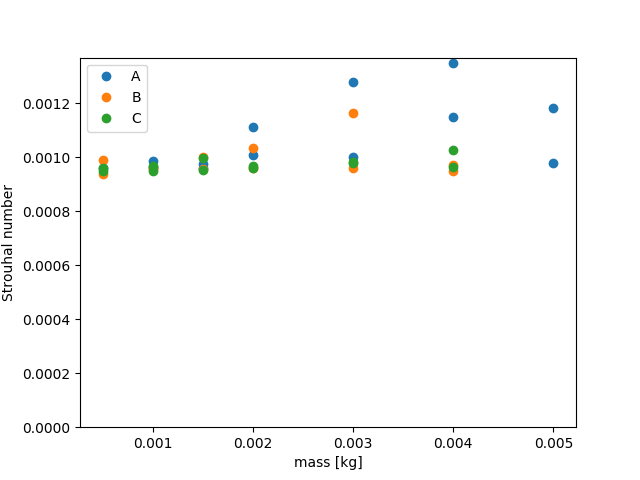
\includegraphics[width=0.8\linewidth]{oppg2.png}
  \caption{
    \label{fig:oppg2}
    Strouhal number of the different seeds
  }
\end{figure}
\subsection{Falling velocity for multiple $\sqrt{W}$}
From the results it is evident that seed A, which had the least bent wings
had the largest vertical velocity. This is likely because the less angled wings
combined with a smaller spanned area induces less drag and also lift on the
seed. This is also as expected when compared to the expressions for drag and lift
derived above.

The more curved seeds have very similar profiles, however the one with the most
curved wings edged slightly ahead. This is perhaps a bit surprising compared
with theory.
\subsection{Stouchal number for different masses}
By inspection, the Stouchal number for different seeds is almost constant.
Because both $\omega$ and $U_V$ depend on the mass and shape in approximately the same manner,
the Stouchal number (relation of angular and translational velocity) is thus
approximately constant for this type of flow. See the discussion in ~\ref{subsec:moment}.

\subsection{Optimal seed configuration}
In terms of determining an optimal configuration, seed B had the slowest descent
and is therefore determined to be the optimal configuration. From the results
it is also clear that the lower the mass, the lower the falling velocity, which
allows the seeds to be carried further before they hit the ground. As a concluding
remark based on the results, the lowest mass medium curved configuration had the
optimal parameters for maximizing dispersion.
\subsection{Possible error}
The failed retrieval of the falling seeds caused the seed to lose some mass
(some of the small lead balls fell out) during the extraction process. Although
it is pretty certain the right amount of lead balls were replaced after
this failure, there might have been some inaccuracies in the seed mass after that
point.
\blankpage
\end{document}

% Local Variables:
% TeX-engine: luatex
% End:
